\documentclass[12pt,english]{article}
\usepackage[utf8]{inputenc}
\usepackage{babel}
\usepackage[margin=0.5 in]{geometry}
\usepackage{caption}
\usepackage{subfig}
\usepackage{longtable}
\usepackage{natbib}
\linespread{1.15}
\usepackage{tikz}
\usepackage{setspace}
\usepackage{listings}
\usepackage{multirow}
\usepackage{multicol}
\usepackage{csquotes}
\usepackage{blindtext}
\usepackage{hyperref}
% ------
% Fonts and typesetting settings


%\usepackage[sc]{mathpazo}
\usepackage{titling}									
\usepackage{float}
\usepackage{pdflscape}
\usepackage[toc]{appendix}
\renewcommand{\appendixtocname}{Appendices}
%\renewcommand{\appendixsection}{\normalfont\bfseries}
\usepackage{amsmath, amsthm, amssymb,amsfonts}

\newcommand{\subtitle}[1]{%
  \posttitle{%
    \par\end{center}
    \begin{center}\large#1\end{center}
    \vskip0.5em}%
}
\usepackage{amsfonts}
\usepackage{amsmath,amsthm,amssymb, graphicx, multicol, array}
\usepackage{bbm, dsfont}
\usepackage{booktabs}												
\usepackage{natbib}                                                 
\usepackage{graphics,epsfig}						
% -----
\title{\textbf{Problem Set 4}\\Estimation of dynamic discrete choice models}
\author{\textbf{ECON: 880}\\
Nicolas Moreno Arias\\ Olivia Wilkinson\\ Kushal Patel}
\date{}

\begin{document}
\maketitle




\section*{Questions}
The value function is given by:

$$
\begin{aligned}
V\left(i, c, p, \epsilon_{t}\right)= & \max _{a \in\{0,1\}} U(a \mid i, c, p, \epsilon)+\beta \sum_{c^{\prime}, p^{\prime}} E_{\epsilon^{\prime}}\left[V\left(i^{\prime}, c^{\prime}, p^{\prime}, \epsilon^{\prime}\right)\right] \operatorname{Pr}\left(c^{\prime}, p^{\prime} \mid c, p, a\right) \\
\text { s.t. } & i^{\prime}=\min \{\bar{i}, i+a-c\} \\
c^{\prime} & = \begin{cases}0 & \text { With probability } 1 / 2 \\
1 & \text { With probability } 1 / 2\end{cases} \\
p^{\prime} & = \begin{cases}p_{s} & \text { With probability } \pi(p) \\
p_{r} & \text { With probability } 1-\pi(p)\end{cases}
\end{aligned}
$$
\subsection*{Question 1}
Define $\bar{V}(s)=E_{\epsilon}[V(s, \epsilon)]$ (as a Fixed Point):

$$
\begin{aligned}
\bar{V}(s) = & \quad E_{\epsilon}[\max_{a} V(a; i, c, p, \epsilon) + \epsilon(a)]\\
= & \quad  \text{ln}\Big(\sum_{a=0,1}e^{ V(a, i, c, p, \epsilon)}  \Big) + \gamma_{\text{euler}}\\
=& \text{ln}\Big(e^{U(0) + \beta F\left(s^{\prime} \mid s, a=0\right) \bar{V}(s)} + e^{U(1)+ \beta F\left(s^{\prime} \mid s, a=1\right) \bar{V}(s)}  \Big) + \gamma_{\text{euler}}\\
=& \text{ln}\Big(e^{\alpha c\mathbbm{1}_{ i > 0} + \lambda\mathbbm{1}_{c > 0} + \beta F\left(s^{\prime} \mid s, a=0\right)\bar{V}(s)} + e^{\alpha c-p + \beta F\left(s^{\prime} \mid s, a=1\right)\bar{V}(s)}  \Big) + \gamma_{\text{euler}} 
\end{aligned}
$$
The numerical solution for the value function is summarized by the following table:
\begin{table}[]
\centering
\caption{}
\begin{tabular}{|c|c|c|c|c|c|c|c|}
\hline
id & I & C & P & U(0) & U(1) & $\bar{V}(s)$      \\
\hline
0  & 0 & 0 & 4 & 0  & -4 & 61.1278 \\
1  & 1 & 0 & 4 & 0  & -4 & 65.0102 \\
2  & 2 & 0 & 4 & 0  & -4 & 68.4821 \\
3  & 3 & 0 & 4 & 0  & -4 & 71.6687 \\
4  & 4 & 0 & 4 & 0  & -4 & 74.6302 \\
5  & 5 & 0 & 4 & 0  & -4 & 77.3943 \\
6  & 6 & 0 & 4 & 0  & -4 & 79.9588 \\
7  & 7 & 0 & 4 & 0  & -4 & 82.2633 \\
8  & 8 & 0 & 4 & 0  & -4 & 84.0732 \\
9  & 0 & 1 & 4 & -4 & -2 & 58.491  \\
10 & 1 & 1 & 4 & 2  & -2 & 63.1278 \\
11 & 2 & 1 & 4 & 2  & -2 & 67.0102 \\
12 & 3 & 1 & 4 & 2  & -2 & 70.4821 \\
13 & 4 & 1 & 4 & 2  & -2 & 73.6687 \\
14 & 5 & 1 & 4 & 2  & -2 & 76.6302 \\
15 & 6 & 1 & 4 & 2  & -2 & 79.3943 \\
16 & 7 & 1 & 4 & 2  & -2 & 81.9588 \\
17 & 8 & 1 & 4 & 2  & -2 & 84.2633 \\
18 & 0 & 0 & 1 & 0  & -1 & 63.2441 \\
19 & 1 & 0 & 1 & 0  & -1 & 66.8946 \\
20 & 2 & 0 & 1 & 0  & -1 & 70.2031 \\
21 & 3 & 0 & 1 & 0  & -1 & 73.2605 \\
22 & 4 & 0 & 1 & 0  & -1 & 76.1102 \\
23 & 5 & 0 & 1 & 0  & -1 & 78.7659 \\
24 & 6 & 0 & 1 & 0  & -1 & 81.2009 \\
25 & 7 & 0 & 1 & 0  & -1 & 83.2815 \\
26 & 8 & 0 & 1 & 0  & -1 & 84.2775 \\
27 & 0 & 1 & 1 & -4 & 1  & 61.0255 \\
28 & 1 & 1 & 1 & 2  & 1  & 65.2441 \\
29 & 2 & 1 & 1 & 2  & 1  & 68.8946 \\
30 & 3 & 1 & 1 & 2  & 1  & 72.2031 \\
31 & 4 & 1 & 1 & 2  & 1  & 75.2605 \\
32 & 5 & 1 & 1 & 2  & 1  & 78.1102 \\
33 & 6 & 1 & 1 & 2  & 1  & 80.7659 \\
34 & 7 & 1 & 1 & 2  & 1  & 83.2009 \\
35 & 8 & 1 & 1 & 2  & 1  & 85.2815\\
\hline
\end{tabular}
\label{Table1}
\end{table}

\subsection*{Question 2}
Following the algorithm in the slides, we use a frequency estimator and compute the implied value function. We then compare it to that obtained in Question 1. We can see that at 4 decimal points, the differences are zero. If we consider more decimal points, we start seeing very negligible differences. (See Table \ref{Table2}).

\begin{table}[]
\caption{}
\label{Table2}
\centering
\begin{tabular}{|c|c|c|c|c|c|c|c|c|}
\hline
id & I & C & P & $\hat{P}_{0}$  & $\hat{P}_{1}$  & $\bar{V}(s)$     & $\hat{\bar{V}}(s)$    & $\Delta\bar{V}(s)$ \\
\hline
0  & 0 & 0 & 4 & 0.4754 & 0.5246 & 61.1278 & 61.1278 & 0        \\
1  & 1 & 0 & 4 & 0.6085 & 0.3915 & 65.0102 & 65.0102 & 0        \\
2  & 2 & 0 & 4 & 0.6828 & 0.3172 & 68.4821 & 68.4821 & 0        \\
3  & 3 & 0 & 4 & 0.7204 & 0.2796 & 71.6687 & 71.6687 & 0        \\
4  & 4 & 0 & 4 & 0.7725 & 0.2275 & 74.6302 & 74.6302 & 0        \\
5  & 5 & 0 & 4 & 0.8278 & 0.1722 & 77.3943 & 77.3943 & 0        \\
6  & 6 & 0 & 4 & 0.8241 & 0.1759 & 79.9588 & 79.9588 & 0        \\
7  & 7 & 0 & 4 & 0.8182 & 0.1818 & 82.2633 & 82.2633 & 0        \\
8  & 8 & 0 & 4 & 0.999  & 0.001  & 84.0732 & 84.0732 & 0        \\
9  & 0 & 1 & 4 & 0.1146 & 0.8854 & 58.491  & 58.491  & 0        \\
10 & 1 & 1 & 4 & 0.4686 & 0.5314 & 63.1278 & 63.1278 & 0        \\
11 & 2 & 1 & 4 & 0.6111 & 0.3889 & 67.0102 & 67.0102 & 0        \\
12 & 3 & 1 & 4 & 0.6731 & 0.3269 & 70.4821 & 70.4821 & 0        \\
13 & 4 & 1 & 4 & 0.7807 & 0.2193 & 73.6687 & 73.6687 & 0        \\
14 & 5 & 1 & 4 & 0.7429 & 0.2571 & 76.6302 & 76.6302 & 0        \\
15 & 6 & 1 & 4 & 0.8358 & 0.1642 & 79.3943 & 79.3943 & 0        \\
16 & 7 & 1 & 4 & 0.8718 & 0.1282 & 81.9588 & 81.9588 & 0        \\
17 & 8 & 1 & 4 & 0.7273 & 0.2727 & 84.2633 & 84.2633 & 0        \\
18 & 0 & 0 & 1 & 0.001  & 0.999  & 63.2441 & 63.2441 & 0        \\
19 & 1 & 0 & 1 & 0.0672 & 0.9328 & 66.8946 & 66.8946 & 0        \\
20 & 2 & 0 & 1 & 0.0826 & 0.9174 & 70.2031 & 70.2031 & 0        \\
21 & 3 & 0 & 1 & 0.0795 & 0.9205 & 73.2605 & 73.2605 & 0        \\
22 & 4 & 0 & 1 & 0.1538 & 0.8462 & 76.1102 & 76.1102 & 0        \\
23 & 5 & 0 & 1 & 0.2174 & 0.7826 & 78.7659 & 78.7659 & 0        \\
24 & 6 & 0 & 1 & 0.3333 & 0.6667 & 81.2009 & 81.2009 & 0        \\
25 & 7 & 0 & 1 & 0.2857 & 0.7143 & 83.2815 & 83.2815 & 0        \\
26 & 8 & 0 & 1 & 0.999  & 0.001  & 84.2775 & 84.2775 & 0        \\
27 & 0 & 1 & 1 & 0.001  & 0.999  & 61.0255 & 61.0255 & 0        \\
28 & 1 & 1 & 1 & 0.0455 & 0.9545 & 65.2441 & 65.2441 & 0        \\
29 & 2 & 1 & 1 & 0.0522 & 0.9478 & 68.8946 & 68.8946 & 0        \\
30 & 3 & 1 & 1 & 0.1    & 0.9    & 72.2031 & 72.2031 & 0        \\
31 & 4 & 1 & 1 & 0.0968 & 0.9032 & 75.2605 & 75.2605 & 0        \\
32 & 5 & 1 & 1 & 0.1765 & 0.8235 & 78.1102 & 78.1102 & 0        \\
33 & 6 & 1 & 1 & 0.2857 & 0.7143 & 80.7659 & 80.7659 & 0        \\
34 & 7 & 1 & 1 & 0.1667 & 0.8333 & 83.2009 & 83.2009 & 0        \\
35 & 8 & 1 & 1 & 0.3333 & 0.6667 & 85.2815 & 85.2815 & 0 \\
\hline
\end{tabular}

\end{table}

\subsection*{Question 3}
According to the Nested Fixed-Point MLE (NFMLE) explained in slide 22, the log-likelihood function is given by the following expression:
$$
   \begin{aligned}
    \textbf{L}(\lambda) = &  \sum_{i} a_i \ln(P(s_i)) + (1 - a_i) \ln(1 - P(s_i))\\
   & s.t \\
   P(s_i) = &\Psi(s_i) \equiv (1 + e^{-\tilde{{v}}(s_i)^{k-1}})^{-1}
    \end{aligned}
$$
where $\Psi(s_i)$ follows the formula described in Algorithm 2 in the slides, as well as $\tilde{{v}}(s_i)^{k-1}$, which is defined as:
$$
   \begin{aligned}   
   \tilde{{v}}(s_i)^{k-1} = U(1) + \beta F\left(s_i^{\prime} \mid s_i, a_i=1\right)\bar{V}^{k-1} - \Big(U(0) + \beta F\left(s_i^{\prime} \mid s_i, a_i=0\right)\bar{V}^{k-1}\Big)
   \end{aligned}
$$


\subsection*{Question 4}
Using the steps for NFPMLE, we obtained $\hat{\lambda} =-4.02$ and the log-likelihood obtained was $\textbf{L}(\hat{\lambda}) =-2634.741$. The graph \ref{fig1} illustrates the optimization by plotting the log-likelihood over different parameter values and on top of it the blue lines give us the optimal parameter and the corresponding log-likelihood value.

\begin{figure}[ht!]
    \centering
    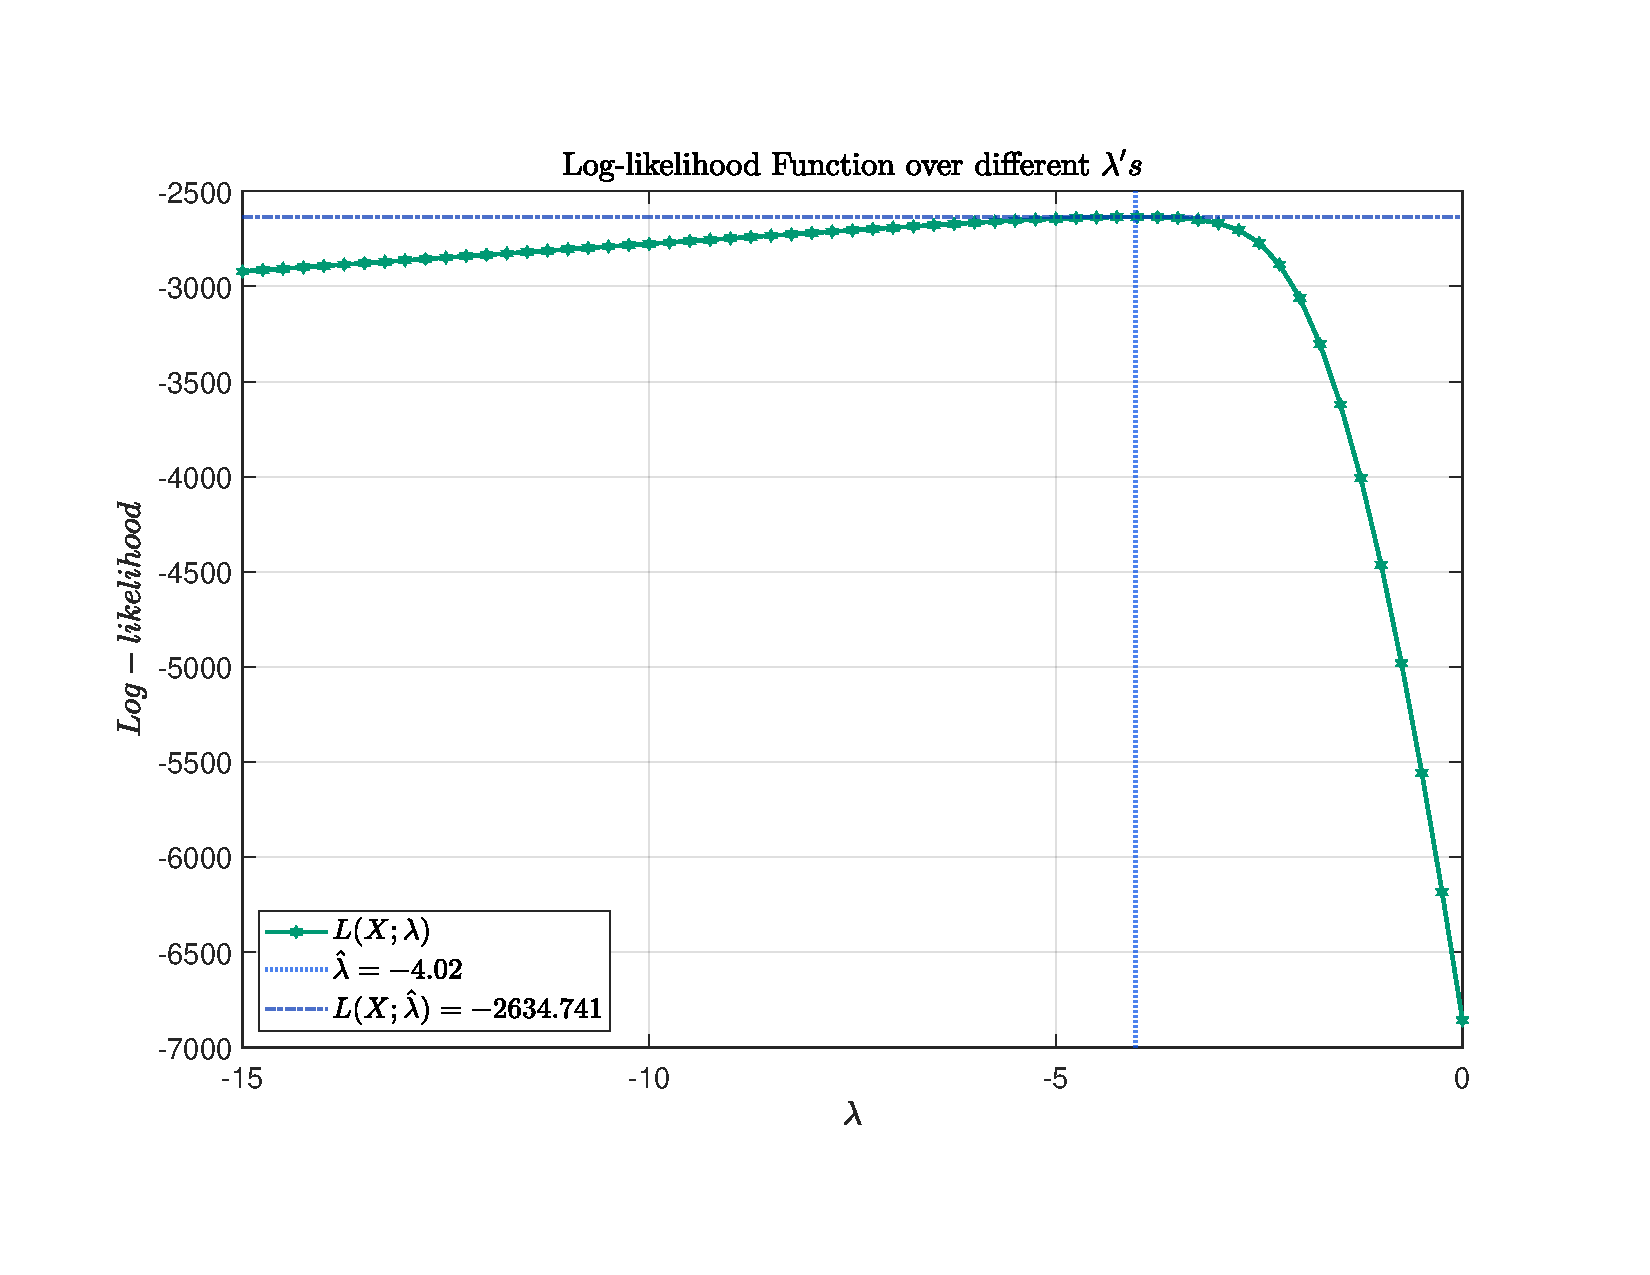
\includegraphics[scale=0.65]{Computational/ECON 880 Q1/Q2/Log-likelihood Function.pdf}
    \vspace{-1cm}
    \caption{}
    \label{fig1}
\end{figure}

   
\end{document}
